% Options for packages loaded elsewhere
\PassOptionsToPackage{unicode}{hyperref}
\PassOptionsToPackage{hyphens}{url}
%
\documentclass[
  12pt,
]{article}
\usepackage{amsmath,amssymb}
\usepackage{lmodern}
\usepackage{iftex}
\ifPDFTeX
  \usepackage[T1]{fontenc}
  \usepackage[utf8]{inputenc}
  \usepackage{textcomp} % provide euro and other symbols
\else % if luatex or xetex
  \usepackage{unicode-math}
  \defaultfontfeatures{Scale=MatchLowercase}
  \defaultfontfeatures[\rmfamily]{Ligatures=TeX,Scale=1}
\fi
% Use upquote if available, for straight quotes in verbatim environments
\IfFileExists{upquote.sty}{\usepackage{upquote}}{}
\IfFileExists{microtype.sty}{% use microtype if available
  \usepackage[]{microtype}
  \UseMicrotypeSet[protrusion]{basicmath} % disable protrusion for tt fonts
}{}
\makeatletter
\@ifundefined{KOMAClassName}{% if non-KOMA class
  \IfFileExists{parskip.sty}{%
    \usepackage{parskip}
  }{% else
    \setlength{\parindent}{0pt}
    \setlength{\parskip}{6pt plus 2pt minus 1pt}}
}{% if KOMA class
  \KOMAoptions{parskip=half}}
\makeatother
\usepackage{xcolor}
\usepackage[margin=1in]{geometry}
\usepackage{graphicx}
\makeatletter
\def\maxwidth{\ifdim\Gin@nat@width>\linewidth\linewidth\else\Gin@nat@width\fi}
\def\maxheight{\ifdim\Gin@nat@height>\textheight\textheight\else\Gin@nat@height\fi}
\makeatother
% Scale images if necessary, so that they will not overflow the page
% margins by default, and it is still possible to overwrite the defaults
% using explicit options in \includegraphics[width, height, ...]{}
\setkeys{Gin}{width=\maxwidth,height=\maxheight,keepaspectratio}
% Set default figure placement to htbp
\makeatletter
\def\fps@figure{htbp}
\makeatother
\setlength{\emergencystretch}{3em} % prevent overfull lines
\providecommand{\tightlist}{%
  \setlength{\itemsep}{0pt}\setlength{\parskip}{0pt}}
\setcounter{secnumdepth}{-\maxdimen} % remove section numbering
\usepackage{pdflscape}
\newcommand{\blandscape}{\begin{landscape}}
\newcommand{\elandscape}{\end{landscape}}
\usepackage{float}
\usepackage{caption}
\usepackage{setspace}\doublespacing
\usepackage{soul}
\floatplacement{figure}{H}
\usepackage{afterpage}
\usepackage{placeins}
\usepackage{graphicx}
\usepackage{floatpag}
\usepackage{float}
\usepackage{booktabs}
\usepackage{longtable}
\usepackage{array}
\usepackage{multirow}
\usepackage{wrapfig}
\usepackage{colortbl}
\usepackage{pdflscape}
\usepackage{tabu}
\usepackage{threeparttable}
\usepackage{threeparttablex}
\usepackage[normalem]{ulem}
\usepackage{makecell}
\usepackage{xcolor}
\ifLuaTeX
  \usepackage{selnolig}  % disable illegal ligatures
\fi
\IfFileExists{bookmark.sty}{\usepackage{bookmark}}{\usepackage{hyperref}}
\IfFileExists{xurl.sty}{\usepackage{xurl}}{} % add URL line breaks if available
\urlstyle{same} % disable monospaced font for URLs
\hypersetup{
  hidelinks,
  pdfcreator={LaTeX via pandoc}}

\author{}
\date{\vspace{-2.5em}}

\begin{document}

\captionsetup[figure]{labelformat=empty}
\captionsetup[table]{labelformat=empty}
\captionsetup[table]{font={stretch=1.2}}

\singlespacing

\vspace{2cm}

\hypertarget{supplementary-information-for}{%
\section{Supplementary information
for:}\label{supplementary-information-for}}

\hypertarget{covariation-among-reproductive-traits-in-flowering-plants-shape-their-interactions-with-pollinators}{%
\subsection{Covariation among reproductive traits in flowering plants
shape their interactions with
pollinators}\label{covariation-among-reproductive-traits-in-flowering-plants-shape-their-interactions-with-pollinators}}

\textbf{Jose B. Lanuza*, Romina Rader, Jamie Stavert, Liam K. Kendall, Manu E. Saunders and Ignasi Bartomeus}

\textbf{*Corresponding author} \textbf{E-mail:
\href{mailto:barragansljose@gmail.com}{\nolinkurl{barragansljose@gmail.com}}}

\textbf{This pdf includes:}

Appendix S1 (text)

Tables S1 to S5

Figures S1 to S9

\doublespacing

\newpage

\hypertarget{appendix-s1}{%
\subsection{Appendix S1}\label{appendix-s1}}

\textbf{Description of the traits compiled in this study}

Here we describe the different individual traits that have been included
in the database:

\emph{Reproductive biology traits}

\begin{itemize}
\item
  Breeding system: All species were classified in hermaphrodite,
  dioecious and monoecious species. Intermediate breeding systems or
  more complex ones were also annotated but all the species were divided
  into these three main categories for simplicity of the analysis.
\item
  Selfing level: We recorded the selfing level of the different species
  with both quantitative and qualitative data. The qualitative data was
  divided in four main categories, high selfers (76\% to 100\% of
  selfing), medium selfers (26\% to 75\%), low selfers (1\% to 25\%) and
  none (0\%) which was for the species that were unable to
  self-pollinate. The quantitative column of selfing had a high
  percentage of missing values (68\%) but we were able to solve this by
  converting the four categories from the qualitative column to
  numerical. For this, we considered the mean value of the different
  categories, that is the categories of `none', `low', `medium' and
  `high' represented 0\%, 13\%, 50.5\% and 88\% of selfing,
  respectively. This reduced the percentage of missing of this column
  from 68\% to 35\% and allowed the imputation of this variable.
\item
  Compatibility system: The different species were divided in three main
  categories in order to know their ability to self-pollinate. These
  categories were self-compatible, partially self-compatible and
  self-incompatible species. The field of selfing level is partly
  complementary to the compatibility system but is important to note
  that not all the self-compatible species or partially self-compatible
  species will self-pollinate.
\end{itemize}

\emph{Floral traits}

\begin{itemize}
\item
  Flower symmetry: Depending on the possible number of identical
  divisions of a flower, plant species were classified into zygomorphic
  (bilaterally symmetrical with only two identical parts) and
  actinomorphic (radially symmetrical with more than three identical
  parts).
\item
  Flower and inflorescence size: We searched for flower length and
  flower and inflorescence width (mm) for all species. When possible, we
  calculated the not found measurements with the help of online images
  and the software ImageJ. Note that for species with compound flowers
  (e.g., Asteraceae) or similar floral structures with flower heads with
  many small flowers we considered the inflorescence as the floral unit.
  For each species this is indicated in the dataset with the field of
  ``info\_level'' where the measurement level is specified as capitulum
  or flower level. Note that for some Asteraceae species information
  about the disc and ray floret is also provided in the database but
  these were not included in our analyses.
\item
  Flower number per plant: We compiled information about the number of
  flowers per plant for all species. However, this field was rare to
  find and we also used online images of the different species in order
  to calculate rough numbers of flowers per plant. We referenced all the
  filled fields in order to be able to follow the images that were used
  for these counts. It is important to note, that these numbers are not
  pretended to be the exact number of flowers per species but an
  approximate indicator of the reproductive investment for the different
  species that allow the macroecological analysis of this field.
\item
  Ovule number: We searched for the number of ovules per flower for all
  the different species. The number of ovules of Asteraceae species are
  considered as the total number of ovules per capitulum. Many species
  were filled by genus or family level because the number of ovules of
  some taxonomic groups is considered to be mostly constant (e.g.,
  Lamiaceae, Boraginaceae or Apiaceae).
\item
  Flower morphology: We looked for images and illustrations of the
  flowers from the different species on the floras and available
  resources in order to categorize the flower shape. We divided the
  flowers in 8 main different categories: open, bowl, tube, campanulate,
  funnelform, papilionaceous, brush and capitulum. However, we ended up
  groupping all flowers on the following 6 morphological groups for
  analyses: tube, papilonaceous, open, capitulum, campanulate and brush
  (Supplementary Information Text Fig. 1).
\end{itemize}

\begin{figure}[h]

{\centering \includegraphics[width=0.65\linewidth,]{../Images/flower_shapes} 

}

\caption{\textbf{Supplementary Information Text Fig. 1.}  Main floral morphologies considered in this study. All species were groupped within these categories for analysis: (a) tube, (b) papilonaceous, (c) open, (d) capitulum, (e) campanulate and (f) brush.}\label{fig:pressure}
\end{figure}

\begin{itemize}
\item
  Style length: We searched for the length of the style (the pistil
  excluding the ovary and the stigma) in millimeters for all plant
  species. When the information about style length was missing, we tried
  to calculate it from images and illustrations from online resources
  (e.g., floras).
\item
  Nectar provision: We recorded the presence and absence of nectar for
  all species. In addition, we also searched for microlitres and
  milligrams of nectar per flower. For species that did not have nectar
  information but belonged to a family that is considered as
  `nectarless', this trait was recorded at family level and the species
  was recorded with `absence' of nectar. This was done exclusively for
  well documented nectarless taxonomical groups. For the field of
  microlitres of nectar, we considered single measurements of nectar
  standing crop. Despite the timing and methodology of the different
  quantitative measurements of nectar differed across studies, these
  fields allowed us to have an approximate idea of the reproductive
  investment of the different plant species.
\item
  Pollen grains per flower: For each species, we searched for the total
  number of pollen grains per flower. Because this fields was rarely
  available, we also tried to recover from pollen:ovule ratio
  information the total number of pollen grains by multiplying it by the
  average ovule number found for each species.
\end{itemize}

\emph{Other life history traits}

\begin{itemize}
\tightlist
\item
  Life form, life span and plant height: We divided the different plant
  species in 4 main categories: herbs, vines, shrubs and trees.
  Moreover, we also divided the species between short-lived species
  (annual, biennial and short-lived perennials) and perennial species
  (long-lived). Finally, we also searched for the average height (m) of
  the different species and annotated the maximum and minimum height
  when possible. We conducted the average between the maximum and
  minimum height to get an approximate average height of the species
  when the average was not indicated.
\end{itemize}

\begin{landscape}


\begingroup\fontsize{12}{14}\selectfont

\begin{longtable}[l]{lrlll}
\caption{\label{tab:unnamed-chunk-2}\textbf{Table S1. List of the 28 plant-pollinator studies used to build the plant trait database. Each study is shown with the first author that conducted the study, number of networks or metawebs that contains, type of information that contains (weighted or unweighted),  the structure (web or metaweb), year of publication and digital object identifier or permanent link for each study.}}\\
\toprule
First author & Year & Web N. & Network type & DOI\\
\midrule
\endfirsthead
\caption[]{\textit{(continued)}}\\
\toprule
First author & Year & Web N. & Network type & DOI\\
\midrule
\endhead

\endfoot
\bottomrule
\endlastfoot
\cellcolor{gray!6}{Arroyo-Correa} & \cellcolor{gray!6}{2019} & \cellcolor{gray!6}{3} & \cellcolor{gray!6}{Weighted web} & \cellcolor{gray!6}{https://doi.org/10.1111/1365-2745.13332}\\
\addlinespace
Bartomeus & 2008 & 6 & Weighted web & https://doi.org/10.1007/s00442-007-0946-1\\
\addlinespace
\cellcolor{gray!6}{Bartomeus} & \cellcolor{gray!6}{2008} & \cellcolor{gray!6}{16} & \cellcolor{gray!6}{Weighted web} & \cellcolor{gray!6}{https://github.com/ibartomeus/BeeFunData}\\
\addlinespace
Bek & 2006 & 1 & Unweighted web & Unpublished, Master thesis\\
\addlinespace
\cellcolor{gray!6}{Bundgaard} & \cellcolor{gray!6}{2003} & \cellcolor{gray!6}{1} & \cellcolor{gray!6}{Weighted web} & \cellcolor{gray!6}{Unpublished, Master thesis}\\
\addlinespace
Burkle & 2013 & 1 & Weighted web & https://doi.org/10.1126/science.1232728\\
\addlinespace
\cellcolor{gray!6}{Dicks} & \cellcolor{gray!6}{2002} & \cellcolor{gray!6}{2} & \cellcolor{gray!6}{Weighted web} & \cellcolor{gray!6}{https://doi.org/10.1046/j.0021-8790.2001.00572.x}\\
\addlinespace
Dupont & 2003 & 3 & Weighted web & https://doi.org/10.1111/j.1365-2656.2008.01501.x\\
\addlinespace
\cellcolor{gray!6}{Elberling} & \cellcolor{gray!6}{1999} & \cellcolor{gray!6}{1} & \cellcolor{gray!6}{Weighted web} & \cellcolor{gray!6}{https://doi.org/10.1111/j.1600-0587.1999.tb00507.x}\\
\addlinespace
Fang & 2008 & 1 & Weighted web & https://doi.org/10.1111/1749-4877.12190\\
\addlinespace
\cellcolor{gray!6}{Inouye} & \cellcolor{gray!6}{1988} & \cellcolor{gray!6}{1} & \cellcolor{gray!6}{Weighted web} & \cellcolor{gray!6}{https://doi.org/10.1111/j.1442-9993.1988.tb00968.x}\\
\addlinespace
Inouye & 1990 & 1 & Weighted metaweb & http://hdl.handle.net/2433/156099\\
\addlinespace
\cellcolor{gray!6}{Kaiser-Bunbury} & \cellcolor{gray!6}{2017} & \cellcolor{gray!6}{8} & \cellcolor{gray!6}{Weighted web} & \cellcolor{gray!6}{https://doi.org/10.1038/nature21071}\\
\addlinespace
Kaiser-Bunbury & 2011 & 6 & Weighted web & https://doi.org/10.1111/j.1365-2745.2010.01732.x\\
\addlinespace
\cellcolor{gray!6}{Kaiser-Bunbury} & \cellcolor{gray!6}{2010} & \cellcolor{gray!6}{2} & \cellcolor{gray!6}{Weighted web} & \cellcolor{gray!6}{https://doi.org/10.1016/j.ppees.2009.04.001}\\
\addlinespace
Kato & 2000 & 1 & Unweighted web & http://hdl.handle.net/2433/156116\\
\addlinespace
\cellcolor{gray!6}{Kevan} & \cellcolor{gray!6}{1970} & \cellcolor{gray!6}{1} & \cellcolor{gray!6}{Unweighted web} & \cellcolor{gray!6}{https://doi.org/10.2307/2258569}\\
\addlinespace
Lundgren & 2005 & 1 & Weighted web & https://doi.org/10.1657/1523-0430(2005)037[0514:TDAHCW]2.0.CO;2\\
\addlinespace
\cellcolor{gray!6}{McMullen} & \cellcolor{gray!6}{1993} & \cellcolor{gray!6}{1} & \cellcolor{gray!6}{Unweighted metaweb} & \cellcolor{gray!6}{https://biostor.org/reference/244737}\\
\addlinespace
Olesen & 2002 & 2 & Weighted web & https://doi.org/10.1046/j.1472-4642.2002.00148.x\\
\addlinespace
\cellcolor{gray!6}{Peralta} & \cellcolor{gray!6}{2006} & \cellcolor{gray!6}{4} & \cellcolor{gray!6}{Weighted web} & \cellcolor{gray!6}{https://doi.org/10.1111/ele.13510}\\
\addlinespace
Primack & 1983 & 3 & Unweighted metaweb & https://doi.org/10.1080/0028825X.1983.10428561\\
\addlinespace
\cellcolor{gray!6}{Ramirez} & \cellcolor{gray!6}{1989} & \cellcolor{gray!6}{1} & \cellcolor{gray!6}{Unweighted web} & \cellcolor{gray!6}{https://doi.org/10.2307/2388282}\\
\addlinespace
Ramirez & 1992 & 1 & Unweighted metaweb & https://doi.org/10.1111/j.1095-8339.1992.tb00294.x\\
\addlinespace
\cellcolor{gray!6}{Robertson} & \cellcolor{gray!6}{1929} & \cellcolor{gray!6}{1} & \cellcolor{gray!6}{Unweighted metaweb} & \cellcolor{gray!6}{https://doi.org/10.5962/bhl.title.11538}\\
\addlinespace
Small & 1976 & 1 & Weighted web & /13960/t4km08d21\\
\addlinespace
\cellcolor{gray!6}{Souza} & \cellcolor{gray!6}{2017} & \cellcolor{gray!6}{1} & \cellcolor{gray!6}{Weighted web} & \cellcolor{gray!6}{https://doi.org/10.1111/1365-2745.12978}\\
\addlinespace
Traveset & 2013 & 1 & Weighted metaweb & https://doi.org/10.1098/rspb.2012.3040\\*
\end{longtable}
\endgroup{}

\end{landscape}

\pagebreak

\begingroup\fontsize{12}{14}\selectfont

\begin{longtable}[t]{lrrrl}
\caption{\label{tab:unnamed-chunk-3}\textbf{Table S2. Statistical association between the different categorical variables and the first three main axes of trait variation with the full set of species.}}\\
\toprule
Functional traits & Sum Sq & F value & Pr(>F) & PC\\
\midrule
\endfirsthead
\caption[]{\textbf{Table S2. Statistical association between the different categorical variables and the first three main axes of trait variation with the full set of species.} \textit{(continued)}}\\
\toprule
Functional traits & Sum Sq & F value & Pr(>F) & PC\\
\midrule
\endhead

\endfoot
\bottomrule
\endlastfoot
\cellcolor{gray!6}{Breeding system} & \cellcolor{gray!6}{304.59} & \cellcolor{gray!6}{119.50} & \cellcolor{gray!6}{0.00} & \cellcolor{gray!6}{PC1}\\
\addlinespace
Compatibility system & 89.12 & 23.31 & 0.00 & PC1\\
\addlinespace
\cellcolor{gray!6}{Lifespan} & \cellcolor{gray!6}{35.65} & \cellcolor{gray!6}{27.97} & \cellcolor{gray!6}{0.00} & \cellcolor{gray!6}{PC1}\\
\addlinespace
Life form & 565.87 & 222.00 & 0.00 & PC1\\
\addlinespace
\cellcolor{gray!6}{Flower shape} & \cellcolor{gray!6}{132.24} & \cellcolor{gray!6}{20.75} & \cellcolor{gray!6}{0.00} & \cellcolor{gray!6}{PC1}\\
\addlinespace
Flower symmetry & 0.37 & 0.29 & 0.59 & PC1\\
\addlinespace
\cellcolor{gray!6}{Nectar provision} & \cellcolor{gray!6}{0.38} & \cellcolor{gray!6}{0.29} & \cellcolor{gray!6}{0.59} & \cellcolor{gray!6}{PC1}\\
\addlinespace
Breeding system & 304.59 & 119.50 & 0.00 & PC2\\
\addlinespace
\cellcolor{gray!6}{Compatibility system} & \cellcolor{gray!6}{89.12} & \cellcolor{gray!6}{23.31} & \cellcolor{gray!6}{0.00} & \cellcolor{gray!6}{PC2}\\
\addlinespace
Lifespan & 35.65 & 27.97 & 0.00 & PC2\\
\addlinespace
\cellcolor{gray!6}{Life form} & \cellcolor{gray!6}{565.87} & \cellcolor{gray!6}{222.00} & \cellcolor{gray!6}{0.00} & \cellcolor{gray!6}{PC2}\\
\addlinespace
Flower shape & 132.24 & 20.75 & 0.00 & PC2\\
\addlinespace
\cellcolor{gray!6}{Flower symmetry} & \cellcolor{gray!6}{0.37} & \cellcolor{gray!6}{0.29} & \cellcolor{gray!6}{0.59} & \cellcolor{gray!6}{PC2}\\
\addlinespace
Nectar provision & 0.38 & 0.29 & 0.59 & PC2\\*
\end{longtable}
\endgroup{}

\pagebreak

\begingroup\fontsize{12}{14}\selectfont

\begin{longtable}[t]{lrrr}
\caption{\label{tab:unnamed-chunk-4}\textbf{Table S3. Loadings of the first three axes of trait variation of the phylogenetic informed principal component analysis with the full set of species.}}\\
\toprule
  & PC1 & PC2 & PC3\\
\midrule
\endfirsthead
\caption[]{\textbf{Table S3. Loadings of the first three axes of trait variation of the phylogenetic informed principal component analysis with the full set of species.} \textit{(continued)}}\\
\toprule
  & PC1 & PC2 & PC3\\
\midrule
\endhead

\endfoot
\bottomrule
\endlastfoot
\cellcolor{gray!6}{Autonomous selfing} & \cellcolor{gray!6}{0.03} & \cellcolor{gray!6}{0.85} & \cellcolor{gray!6}{-0.51}\\
\addlinespace
Flowers per plant & 0.75 & -0.27 & -0.24\\
\addlinespace
\cellcolor{gray!6}{Flower width} & \cellcolor{gray!6}{-0.67} & \cellcolor{gray!6}{-0.38} & \cellcolor{gray!6}{-0.30}\\
\addlinespace
Style length & -0.34 & -0.37 & -0.66\\
\addlinespace
\cellcolor{gray!6}{Ovule number} & \cellcolor{gray!6}{-0.53} & \cellcolor{gray!6}{0.00} & \cellcolor{gray!6}{-0.02}\\
\addlinespace
Plant height & 0.56 & -0.40 & -0.46\\
\addlinespace
\cellcolor{gray!6}{Explained variation} & \cellcolor{gray!6}{26.72} & \cellcolor{gray!6}{25.08} & \cellcolor{gray!6}{19.17}\\*
\end{longtable}
\endgroup{}

\pagebreak

\begingroup\fontsize{12}{14}\selectfont

\begin{longtable}[t]{lrrr}
\caption{\label{tab:unnamed-chunk-5}\textbf{Table S4. Loadings of the first three axes of trait variation of the phylogenetic informed principal component analysis with the subset of species with data of nectar and pollen quantity.}}\\
\toprule
  & PC1 & PC2 & PC3\\
\midrule
\endfirsthead
\caption[]{\textbf{Table S4. Loadings of the first three axes of trait variation of the phylogenetic informed principal component analysis with the subset of species with data of nectar and pollen quantity.} \textit{(continued)}}\\
\toprule
  & PC1 & PC2 & PC3\\
\midrule
\endhead

\endfoot
\bottomrule
\endlastfoot
\cellcolor{gray!6}{Autonomous selfing} & \cellcolor{gray!6}{-0.05} & \cellcolor{gray!6}{0.78} & \cellcolor{gray!6}{0.37}\\
\addlinespace
Flowers per plant & 0.53 & -0.49 & 0.42\\
\addlinespace
\cellcolor{gray!6}{Flower width} & \cellcolor{gray!6}{-0.74} & \cellcolor{gray!6}{-0.27} & \cellcolor{gray!6}{-0.13}\\
\addlinespace
Style length & -0.60 & -0.30 & 0.11\\
\addlinespace
\cellcolor{gray!6}{Ovule number} & \cellcolor{gray!6}{-0.59} & \cellcolor{gray!6}{0.11} & \cellcolor{gray!6}{-0.08}\\
\addlinespace
Plant height & 0.26 & -0.60 & 0.47\\
\addlinespace
\cellcolor{gray!6}{Microlitres of Nectar per flower} & \cellcolor{gray!6}{-0.49} & \cellcolor{gray!6}{0.05} & \cellcolor{gray!6}{0.71}\\
\addlinespace
Pollen per flower & -0.29 & -0.45 & -0.13\\
\addlinespace
\cellcolor{gray!6}{Explained variation} & \cellcolor{gray!6}{23.42} & \cellcolor{gray!6}{21.13} & \cellcolor{gray!6}{14.84}\\*
\end{longtable}
\endgroup{}

\newpage

\begingroup\fontsize{12}{14}\selectfont

\begin{longtable}[t]{lll}
\caption{\label{tab:unnamed-chunk-6}\textbf{Table S5. Phylogenetic signal of the different quantitative traits.}}\\
\toprule
Functional traits & Lambda & P-value\\
\midrule
\endfirsthead
\caption[]{\textbf{Table S5. Phylogenetic signal of the different quantitative traits.} \textit{(continued)}}\\
\toprule
Functional traits & Lambda & P-value\\
\midrule
\endhead

\endfoot
\bottomrule
\endlastfoot
\cellcolor{gray!6}{Autonomous selfing} & \cellcolor{gray!6}{0.34} & \cellcolor{gray!6}{0.00}\\
\addlinespace
Flower number & 0.69 & 0.00\\
\addlinespace
\cellcolor{gray!6}{Inflorescence width} & \cellcolor{gray!6}{0.57} & \cellcolor{gray!6}{0.00}\\
\addlinespace
Flower width & 0.73 & 0.00\\
\addlinespace
\cellcolor{gray!6}{Flower length} & \cellcolor{gray!6}{0.75} & \cellcolor{gray!6}{0.00}\\
\addlinespace
Style length & 0.49 & 0.00\\
\addlinespace
\cellcolor{gray!6}{Ovule number} & \cellcolor{gray!6}{1.00} & \cellcolor{gray!6}{0.00}\\
\addlinespace
Plant height & 0.96 & 0.00\\
\addlinespace
\cellcolor{gray!6}{Nectar per flower ($\mu$l)} & \cellcolor{gray!6}{0.14} & \cellcolor{gray!6}{0.00}\\
\addlinespace
Nectar concentration ($\%$) & 0.65 & 0.00\\
\addlinespace
\cellcolor{gray!6}{Pollen grains per flower} & \cellcolor{gray!6}{1.00} & \cellcolor{gray!6}{0.00}\\*
\end{longtable}
\endgroup{}

\newpage
\begin{landscape}

\begin{figure}[h]
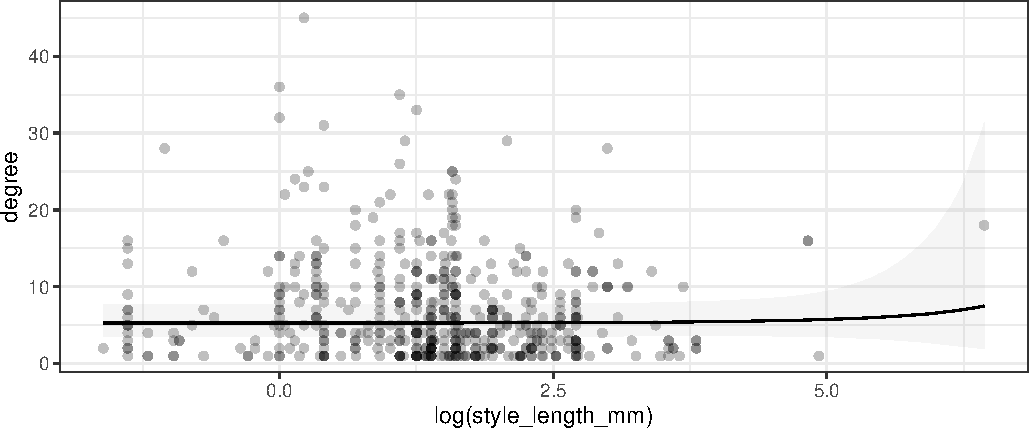
\includegraphics{Sup_Mat_Lanuza_et_al_2022_files/figure-latex/unnamed-chunk-7-1} \caption{\textbf{Fig. S1.} Map with the different locations of the plant-pollinator studies used in this work to explore woldwide patterns at the meso-scale level. Note that for visualization purposes studies from the same authors are shown with the same colour.}\label{fig:unnamed-chunk-7}
\end{figure}

\end{landscape}

\newpage

\begin{figure}[h]
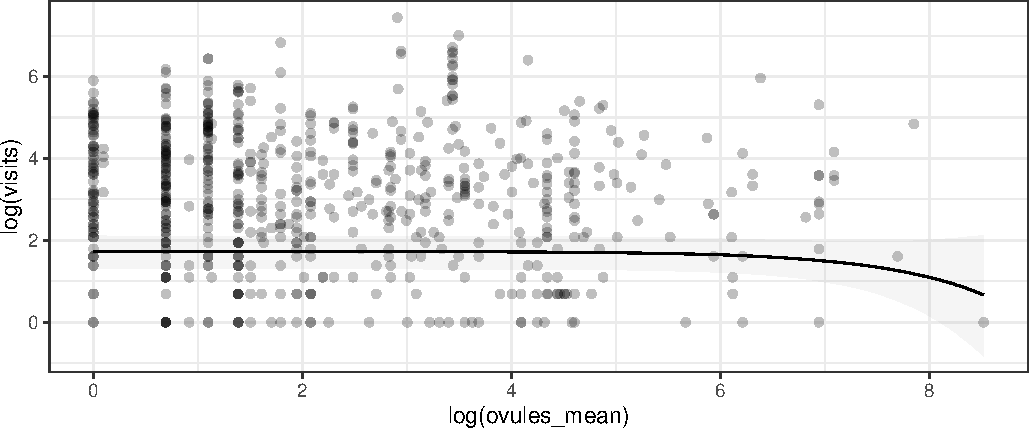
\includegraphics{Sup_Mat_Lanuza_et_al_2022_files/figure-latex/unnamed-chunk-8-1} \caption{\textbf{Fig. S2.} Percentage of present and missing values of the different plant traits.}\label{fig:unnamed-chunk-8}
\end{figure}

\newpage

\begin{figure}[h]

{\centering 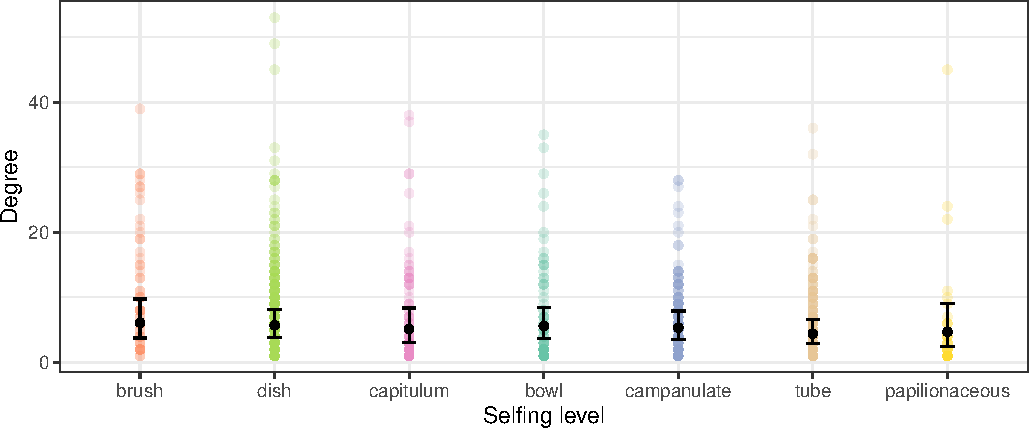
\includegraphics[width=0.6\linewidth,]{Sup_Mat_Lanuza_et_al_2022_files/figure-latex/unnamed-chunk-9-1} 

}

\caption{\textbf{Fig. S3.} Comparison of the phylogenetic informed principal component analysis for the dataset with data imputation and without data imputation. Panel 'a' shows the reproductive spectrum of trait variation for the full dataset with data imputation and panel 'b' shows the reproductive spectrum for the dataset without data imputation where the species with missing trait data were excluded from the analysis.}\label{fig:unnamed-chunk-9}
\end{figure}

\begin{figure}[h]

{\centering 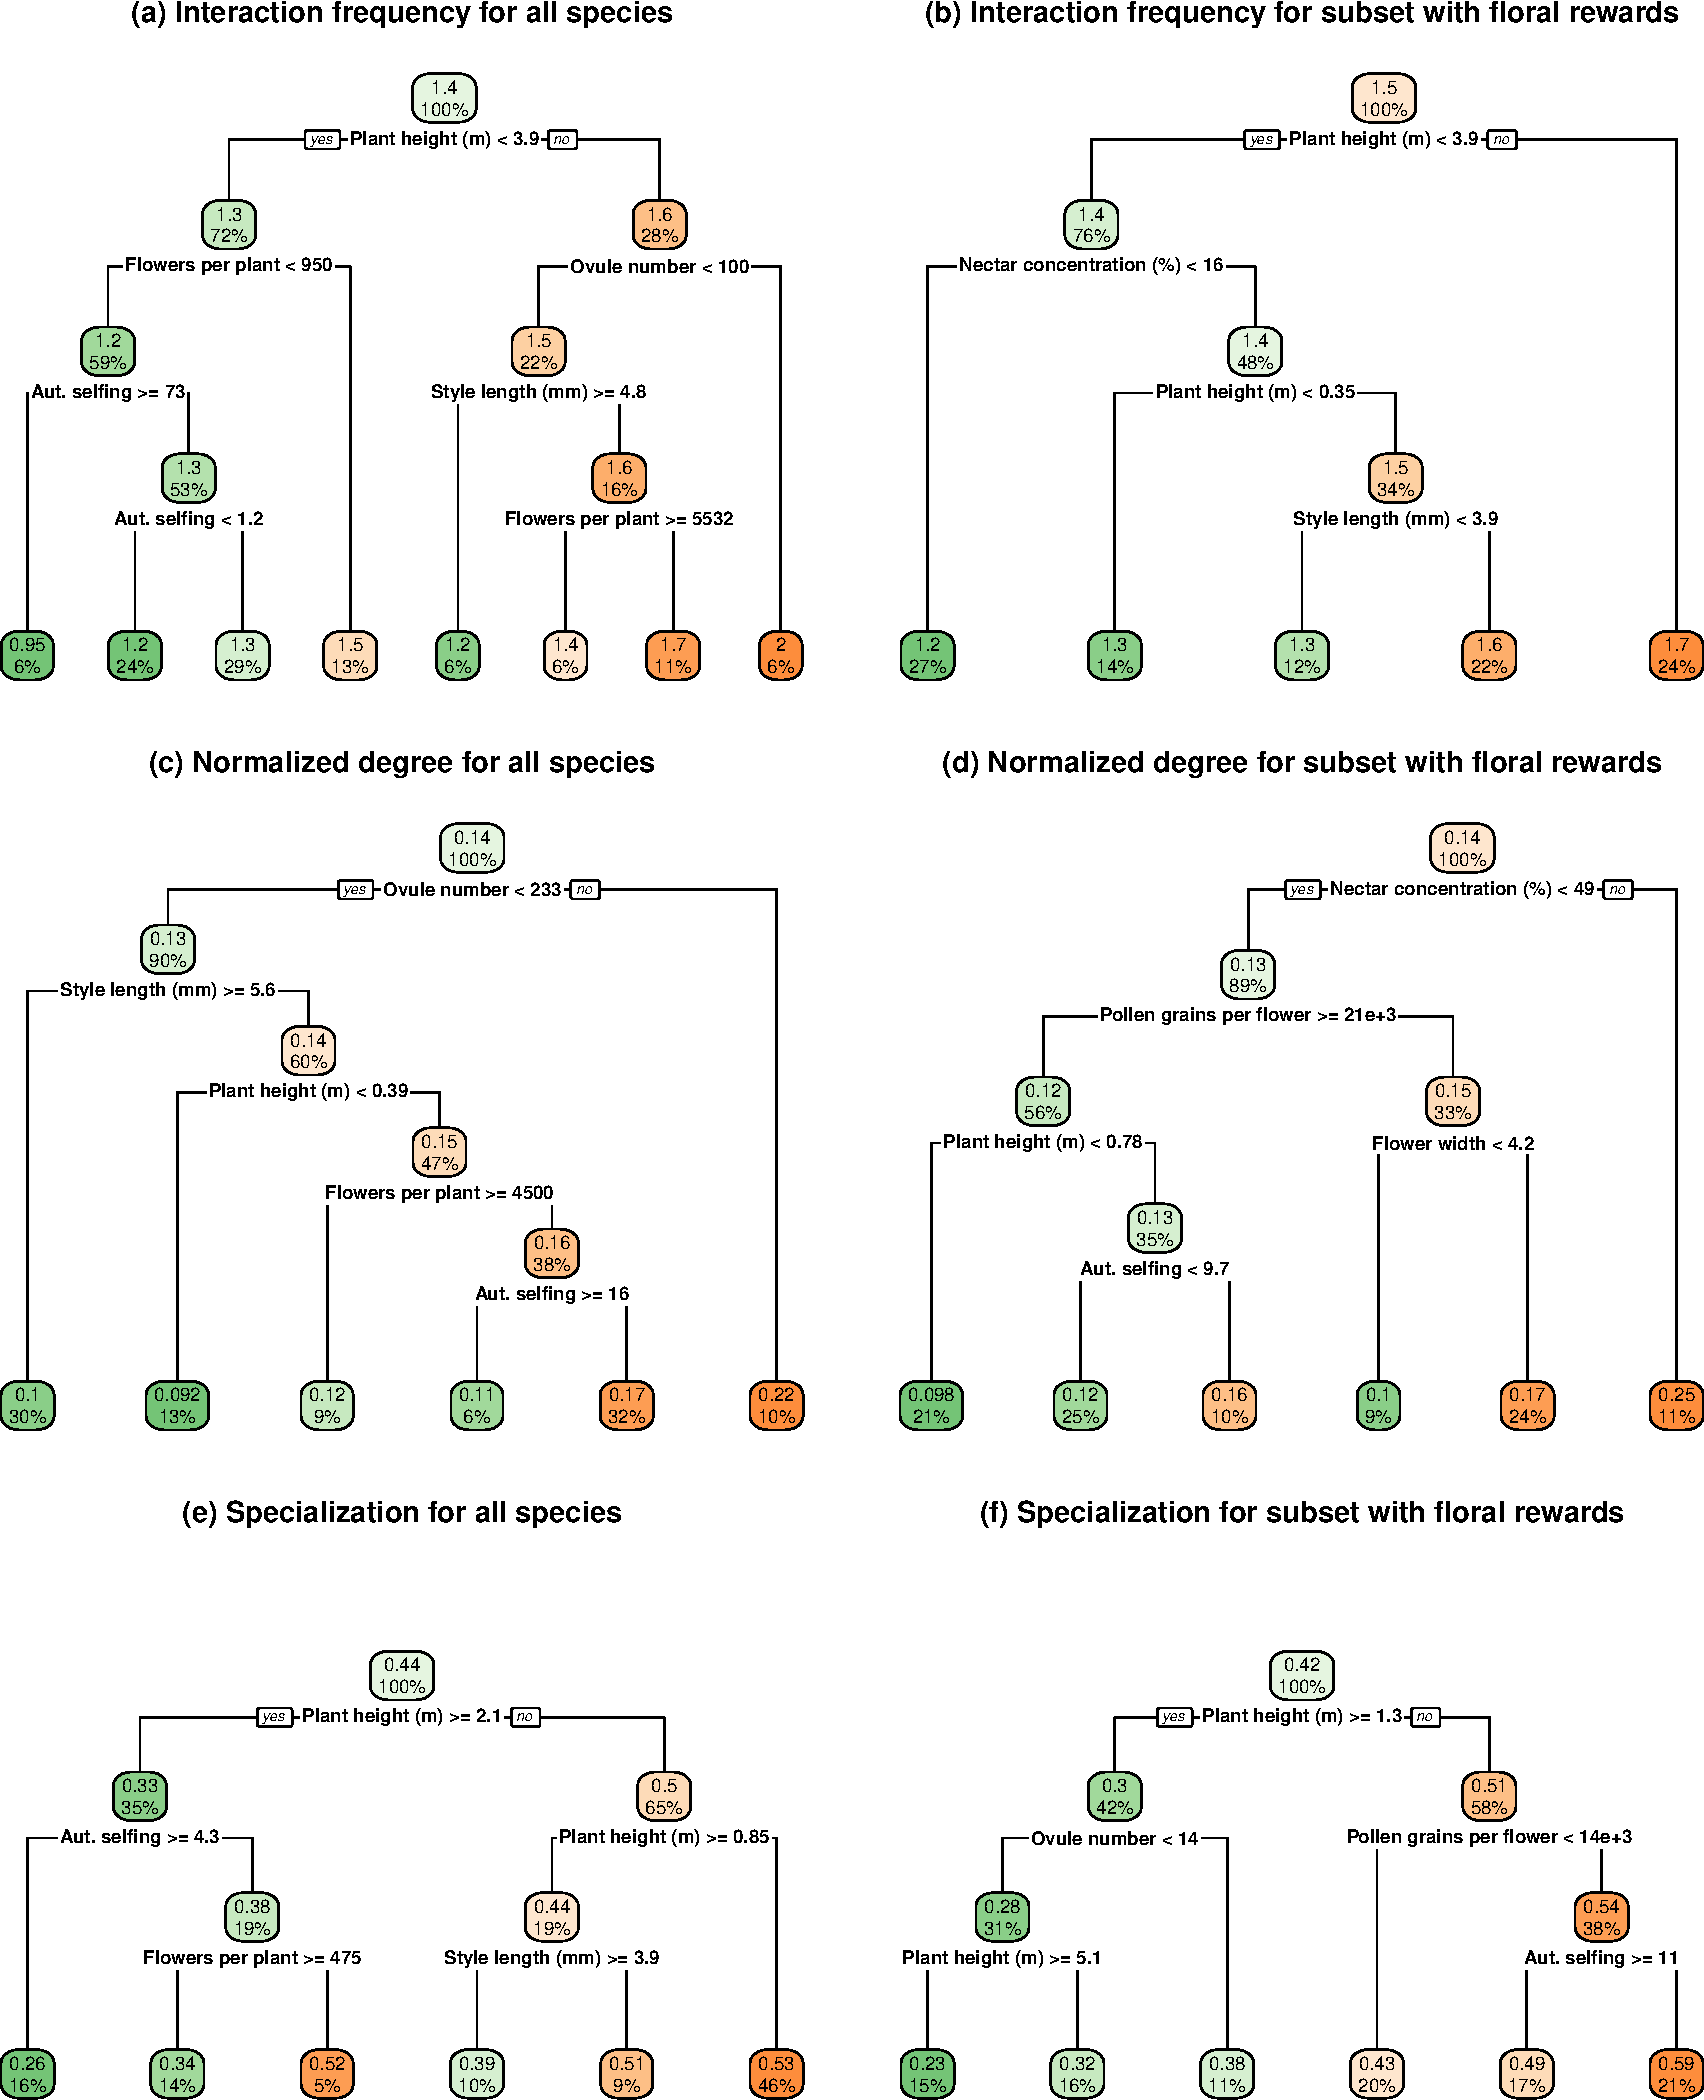
\includegraphics[width=0.6\linewidth,]{Sup_Mat_Lanuza_et_al_2022_files/figure-latex/unnamed-chunk-10-1} 

}

\caption{\textbf{Fig. S4.} Comparison of the phylogenetic informed principal component analysis for the subset of species that had information of floral rewards with data imputation and without data imputation. Panel A shows the reproductive spectrum of trait variation for the dataset with data imputation and panel B shows the reproductive spectrum for the dataset excluding species with missing trait data}\label{fig:unnamed-chunk-10}
\end{figure}

\newpage

\begin{figure}[h]
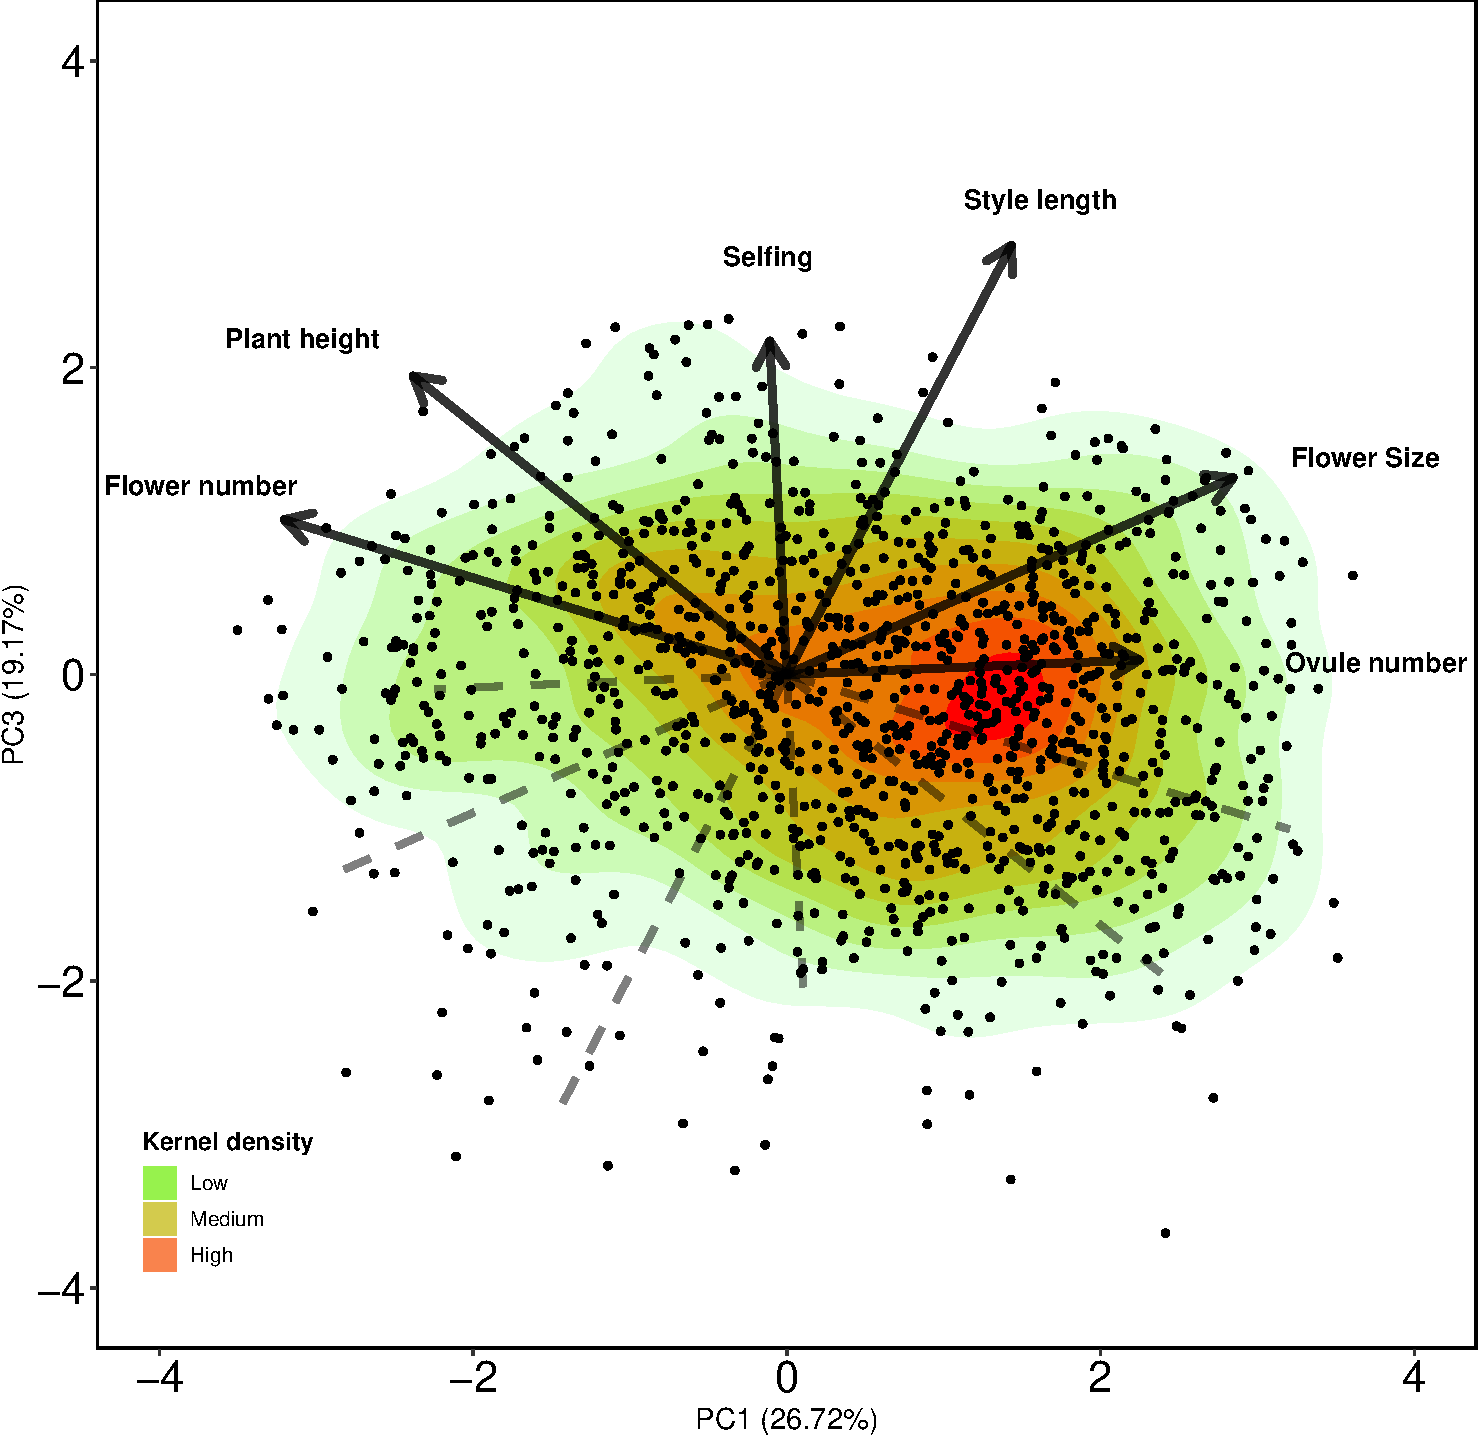
\includegraphics{Sup_Mat_Lanuza_et_al_2022_files/figure-latex/unnamed-chunk-11-1} \caption{\textbf{Fig. S5.} Fitted posterior estimates of the interaction (yes/no) and number of visits made by bees including and exluding honey bees on the main axes of trait variation. The superior panel (plots a, b c, d, e and f) shows the comparison for presence-absence and the lower panel (plots g, h, i, j, k and l) the comparison for visitation rates.}\label{fig:unnamed-chunk-11}
\end{figure}

\newpage

\begin{figure}[h]
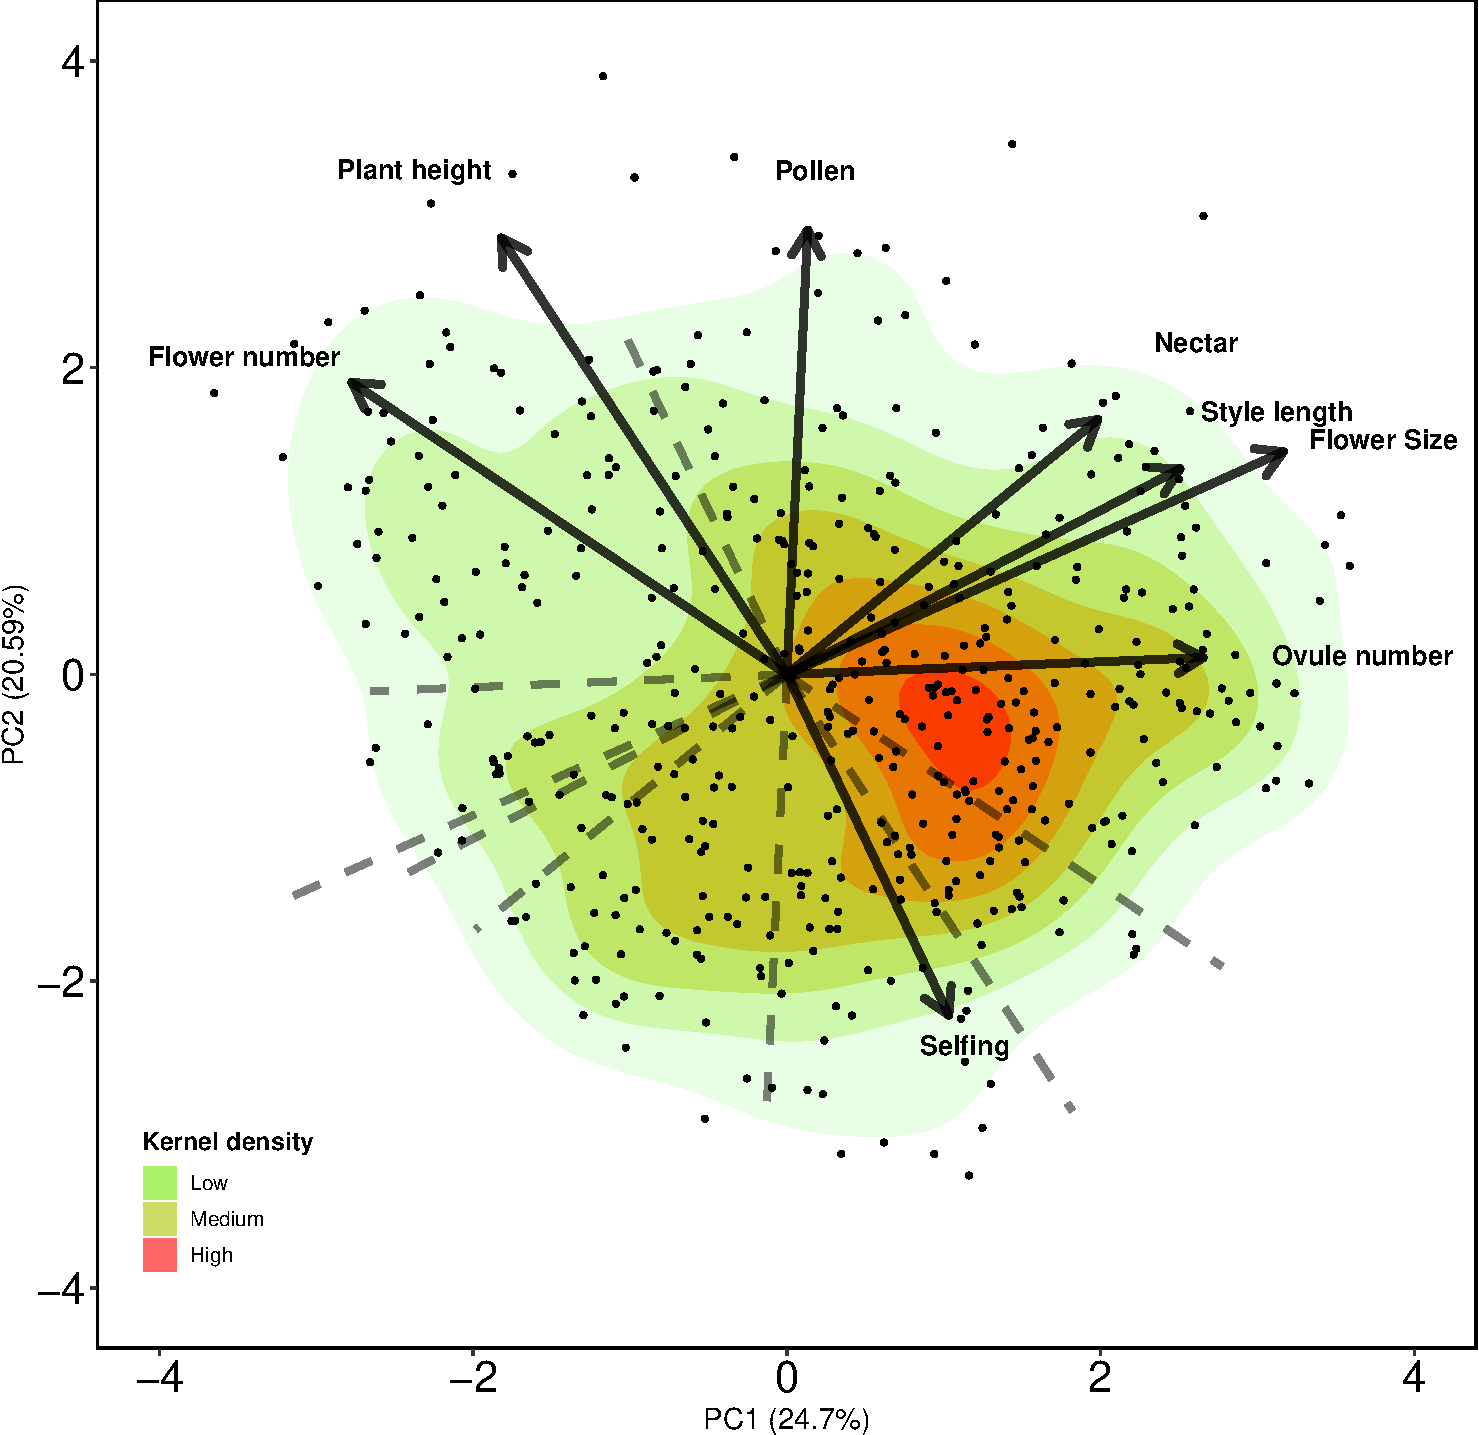
\includegraphics{Sup_Mat_Lanuza_et_al_2022_files/figure-latex/unnamed-chunk-12-1} \caption{\textbf{Fig. S6.} Phylogenetically informed principal component analysis (pPCA) for all plant species with the first (flower number - flower size axis) and third (style length - autonomous selfing) principal component that explained most trait variation.}\label{fig:unnamed-chunk-12}
\end{figure}

\newpage
\thispagestyle{empty}

\begin{figure}[h]
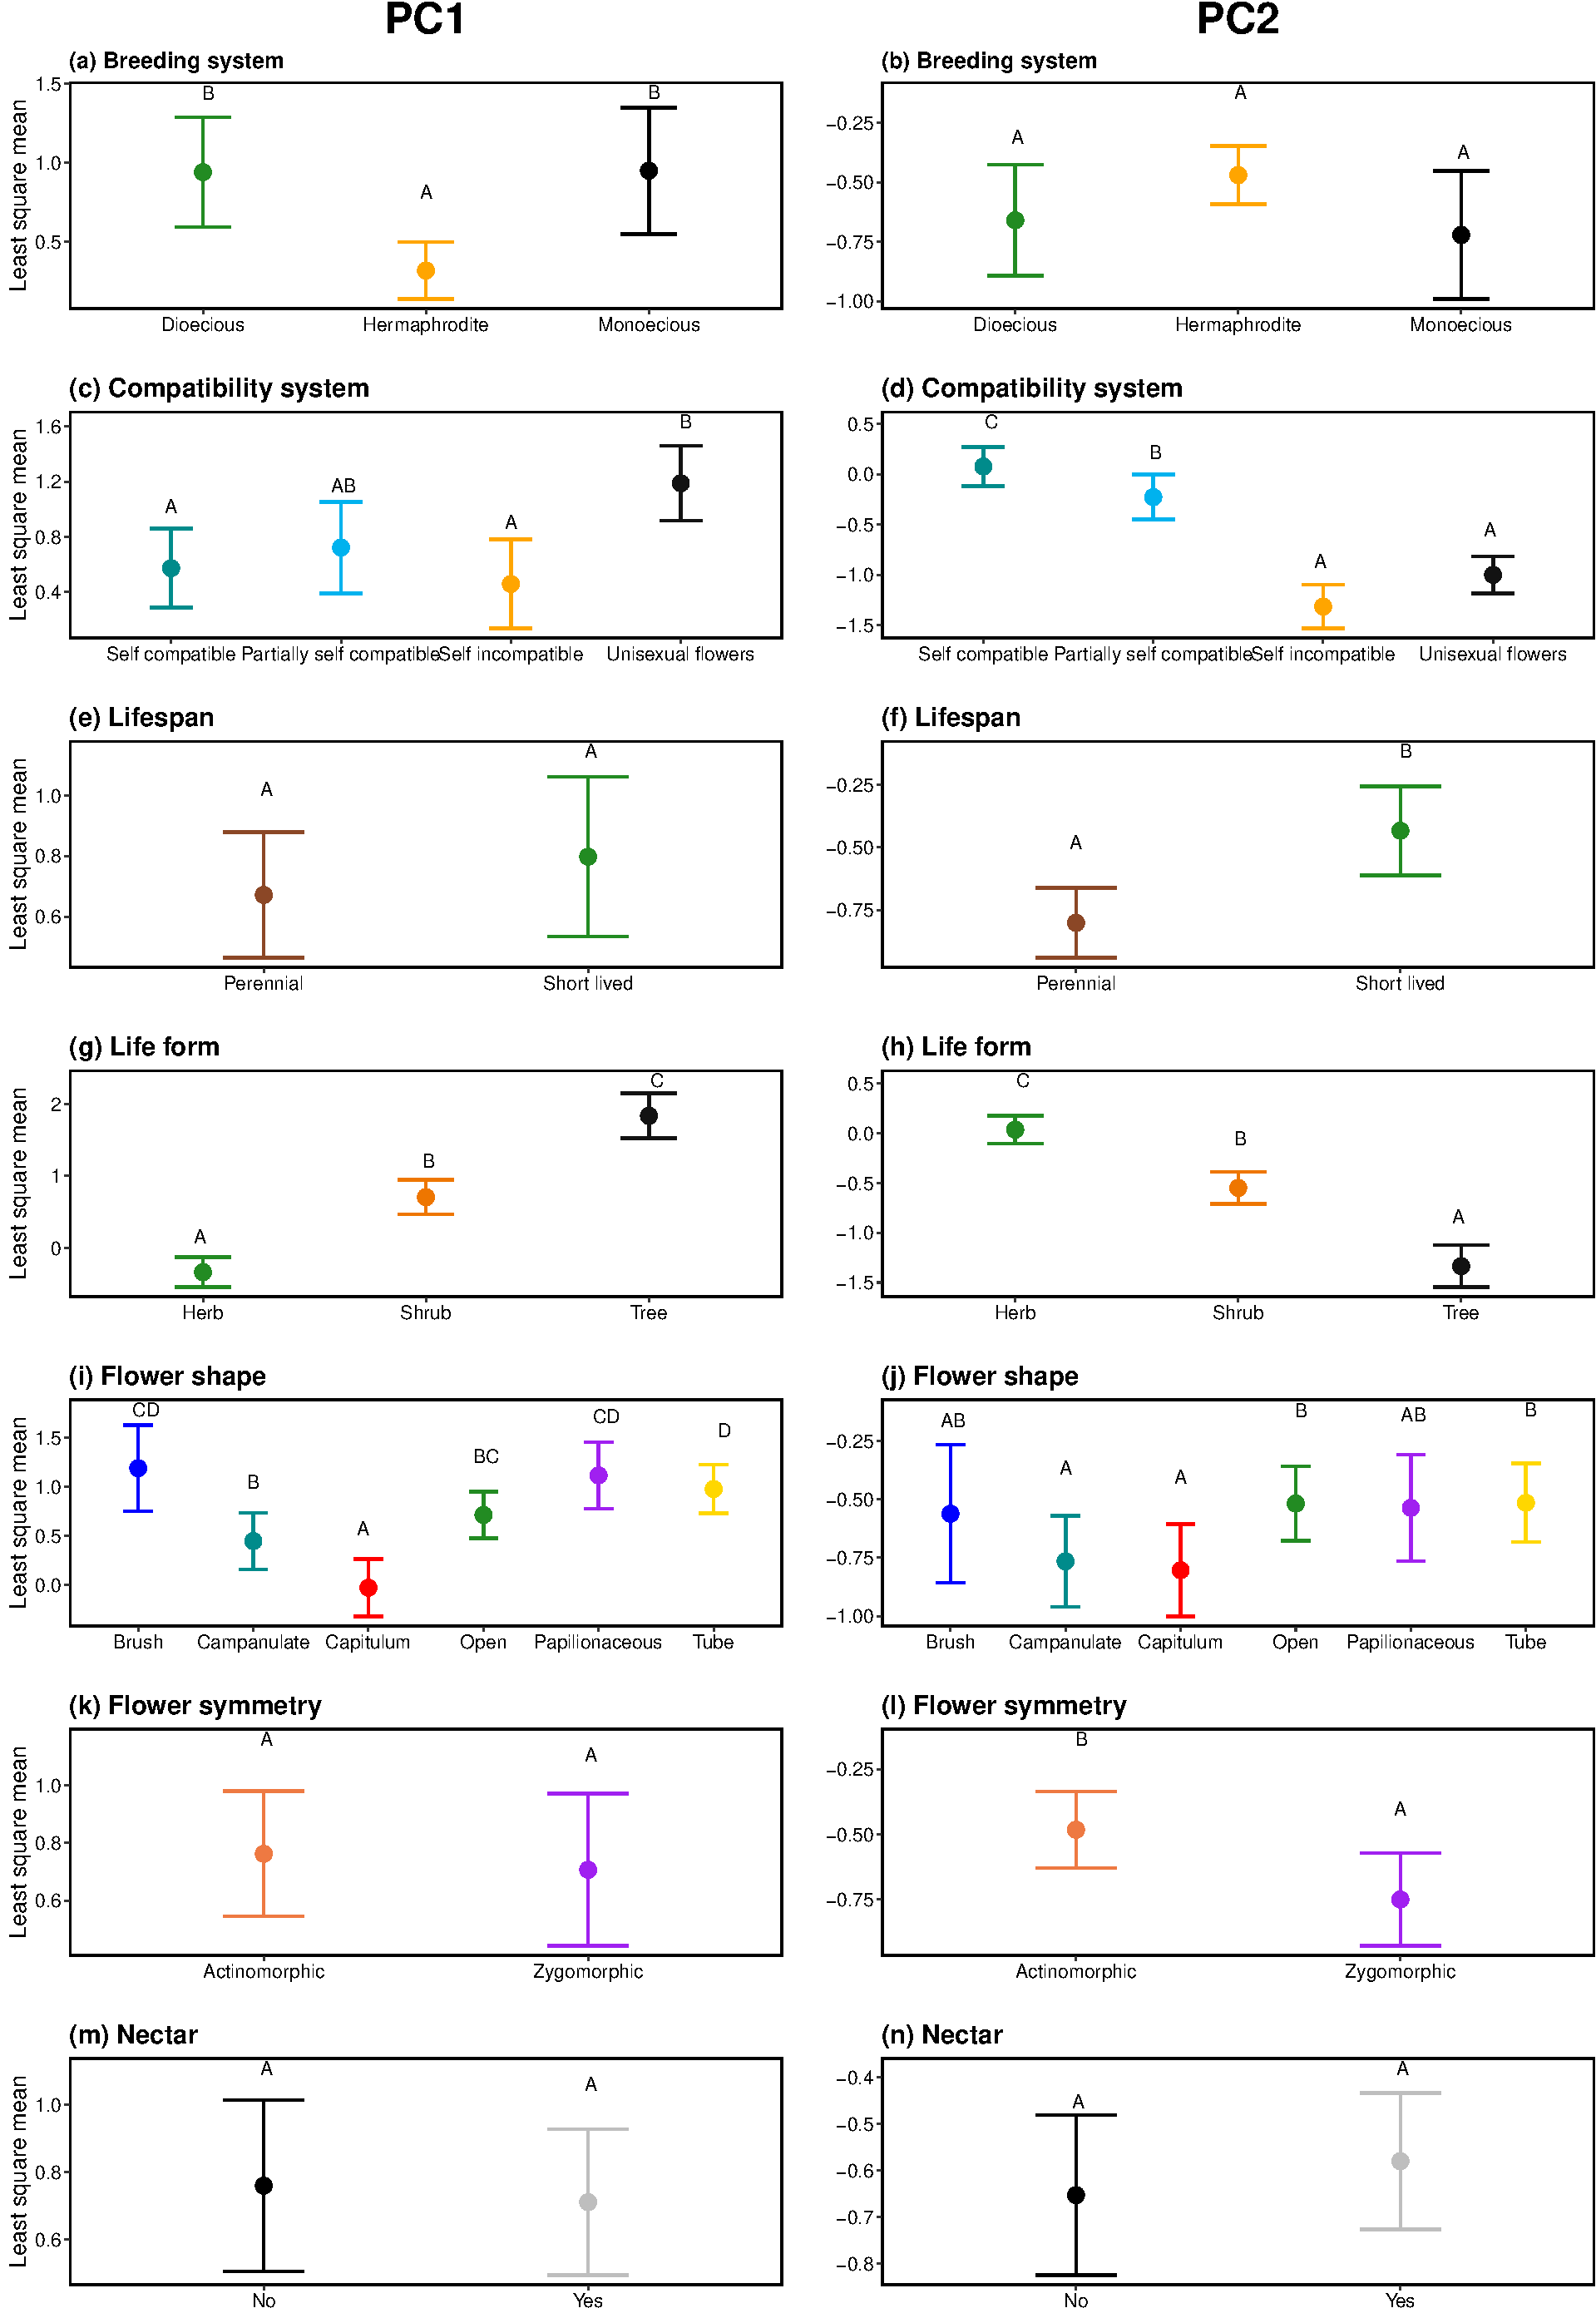
\includegraphics{Sup_Mat_Lanuza_et_al_2022_files/figure-latex/unnamed-chunk-13-1} \caption{\textbf{Fig. S7.} Statistical comparison of the different categories of qualitative traits on the main two axes of trait variation with the full set of species. Categories that differ significantly are denoted with a different letter.}\label{fig:unnamed-chunk-13}
\end{figure}

\begin{landscape}

\begin{figure}[!H]
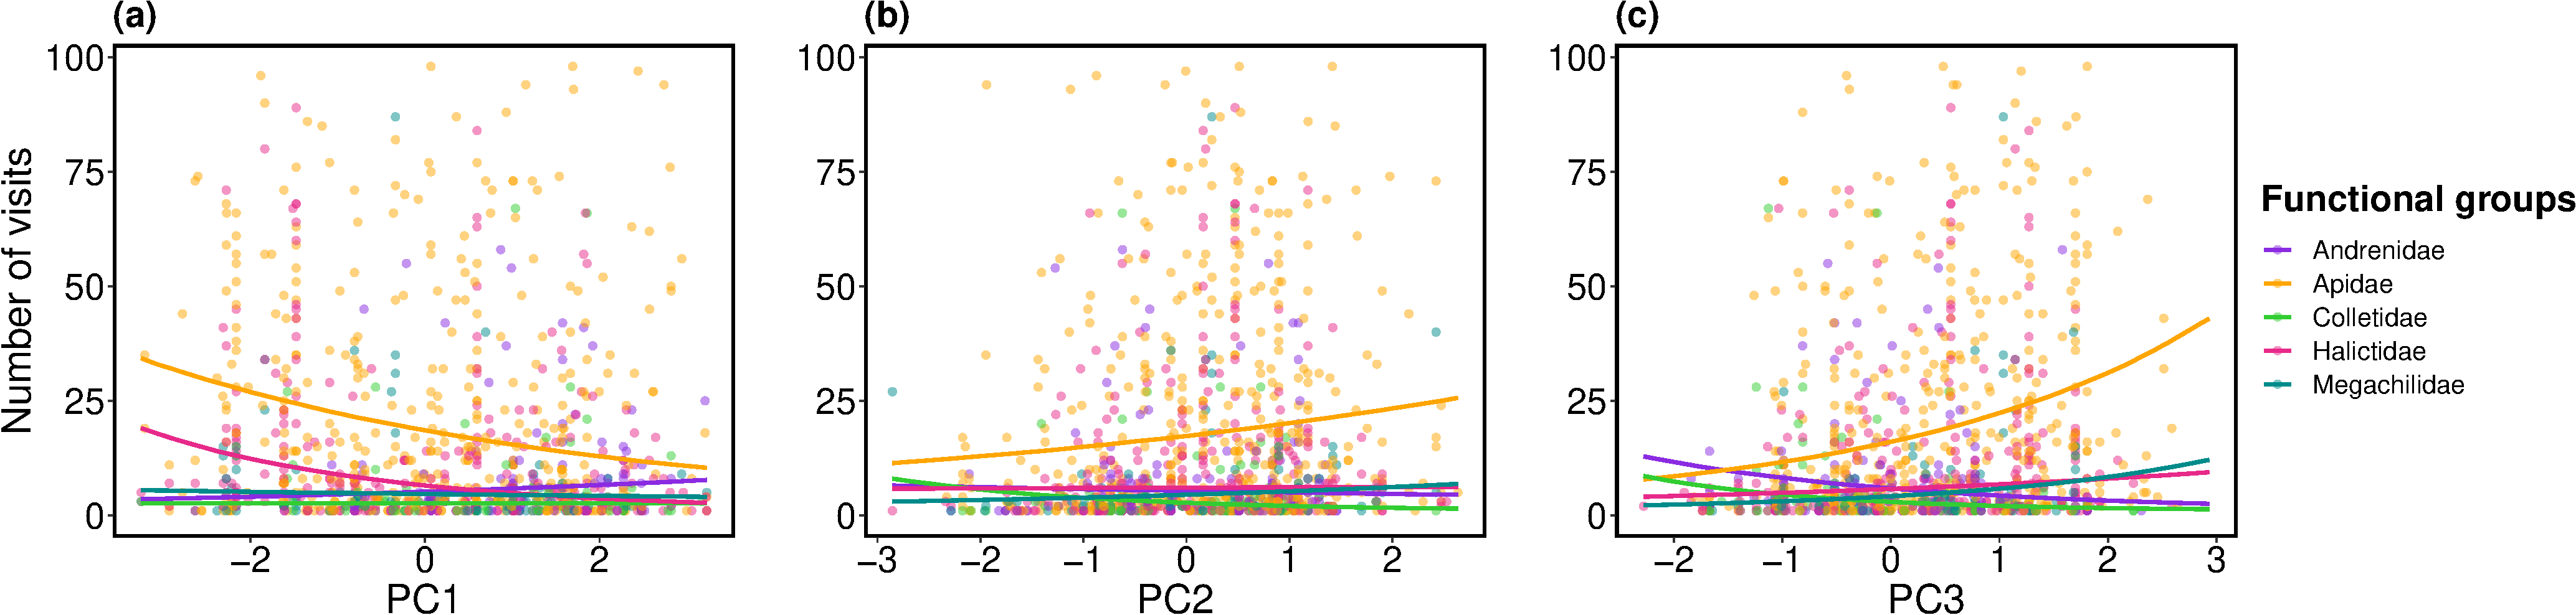
\includegraphics{Sup_Mat_Lanuza_et_al_2022_files/figure-latex/unnamed-chunk-14-1} \caption{\textbf{Fig. S8.} Interaction (yes/no) and visitation rate of the main bee families on the main axes of trait variation. Fitted posterior estimates of the presence-absence of interaction (plots a, b and c) and visitation rate (plots e, f and g) of Andrenidae, Apidae, Colletidae, Halictidae and Megachilidae across PC1, PC2 and PC3. For visualization purposes, the response variable of number of visits was log-transformed (Y-axis of lower panel).}\label{fig:unnamed-chunk-14}
\end{figure}

\end{landscape}

\begin{landscape}

\begin{figure}[h]
\includegraphics{Sup_Mat_Lanuza_et_al_2022_files/figure-latex/unnamed-chunk-15-1} \caption{\textbf{Fig. S9.} Association between the main axes of trait variation (showed on different columns) and the distinct plant species level network metrics (showed on different rows). The x-axis shows the most illustrative trait extremes of the trait continuum. Note that the plots are coloured by the different network metrics.}\label{fig:unnamed-chunk-15}
\end{figure}

\end{landscape}

\end{document}
